\chapter{Metodología}


Este capítulo aborda la metodología empleada en el presente trabajo, la cual se centra en el análisis de tweets relacionados con las elecciones presidenciales en Colombia durante el período de mayo a junio de 2022. El capítulo comienza describiendo la sección de Datos, donde se detalla el proceso de obtención, análisis exploratorio y etiquetado de los datos recopilados. Posteriormente, en la sección de Modelos, se presentan los modelos de lenguaje utilizados y se expone el método correspondiente de entrenamiento y evaluación.

\section{Datos}

En esta sección se aborda la etapa inicial de recolección de datos, llevada a cabo entre la primera y segunda vuelta electoral, utilizando hashtags con contenido político. Luego se detalla el proceso de filtrado aplicado a esta base de datos para retener únicamente los tweets relevantes, seguido de un análisis exploratorio de la información obtenida. También se describe el uso de los hashtags como herramienta para clasificar la orientación política los tweets, basándose en el contenido presente en los tweets que hacen uso de dichos hashtags.

Finalmente, se presenta el proceso de etiquetado manual de emociones en una muestra de los tweets recopilados. Se explica en detalle cómo se llevó a cabo este etiquetado, en el cual se eligieron 14 emociones posibles. Además, se establecen correlaciones entre las etiquetas asignadas por los etiquetadores, lo que resulta en la creación de etiquetas agrupadoras basadas en estas correlaciones. El proceso de asignación a las etiquetas finales para cada tweet se describe en profundidad, y se discute el nivel de acuerdo alcanzado entre los diferentes etiquetadores involucrados en el proceso.



\subsection{Recolección y análisis exploratorio de datos}


El dataset inicialmente recopilado consta de 585,001 tweets obtenidos entre el 22 de mayo y el 22 de junio de 2022, período en el que tuvieron lugar la primera y la segunda vuelta de las elecciones presidenciales en Colombia, el 29 de mayo y el 19 de junio respectivamente. Para la extracción de los datos, se utilizaron 173 tendencias, es decir, hashtags por día, con contenido político que estuvieron presentes durante este lapso. Estos hashtags se obtuvieron de diferentes sitios web \footnote{\url{https://getdaytrends.com/}} \footnote{\url{https://archive.twitter-trending.com/}} \footnote{\url{https://www.exportdata.io/trends/worldwide}}, donde se detallan los hashtags que fueron tendencia en distintos países para fechas específicas. De allí, se seleccionaron los hashtags que estuvieron en tendencia y estaban relacionados con el tema de las elecciones en Colombia durante el periodo de estudio.

El dataset recolectado fue sometido a un proceso de filtrado para eliminar aquellos tweets con menos de 5 palabras, los que tenían una proporción de menciones o hashtags superior al 20\% del total del texto y aquellos que contenían enlaces o provenían de usuarios con un número atípico de publicaciones. Esto redujo la base de datos a 193,348 tweets. A los hashtags utilizados les fue asignada alguna de tres orientaciones políticas: Izquierda, Derecha y Neutro. Esta asignación estuvo basada en la lectura de una muestra de múltiples tweets que contuvieran el hashtag, el contenido asociado a ellos y la inclinación política percibida en términos generales. En el Cuadro \ref{table:hashtags} en la sección de apéndices, se presentan los hashtags junto con su orientación política y la cantidad de tweets asociados a cada uno. A lo largo de este trabajo, cuando se hable de sector político, se hará referencia a esta clasificación.

Cabe destacar que la asignación de un sector político en particular a un hashtag se llevó a cabo a partir de la tendencia política observada en los tweets, y aunque en términos generales los tweets asociados al hashtag presentan cierta inclinación, esto no excluye la presencia de tweets cuya tendencia política sea contraria. En el Cuadro \ref{table:ejemplos_1} se proporcionan ejemplos de tweets que muestran la relación del hashtag con la orientación política. Por ejemplo, el hashtag \#EstallidoSocialEs fue catalogado como de derecha debido a que generalmente presenta tweets como el primer ejemplo. Sin embargo, también existen tweets que lo utilizan para expresar apoyo al candidato de izquierda, como se observa en el segundo ejemplo. De manera similar, el hashtag \#YaEsSuficiente suele ser utilizado mayormente para respaldar a la izquierda, como se ve en el tercer ejemplo. No obstante, también se encuentran casos en los que se utiliza para apoyar a un candidato de derecha, como se muestra en el cuarto ejemplo.


\begin{table}
\caption{Ejemplos de tweets con respecto a orientacion politica}
\label{table:ejemplos_1}
\begin{tabular}{{ | p{2cm} | p{13cm} |}}
\toprule
Numero de Ejemplo & Tweet \\
\midrule
1 & @lcvelez @lafm \#EstallidoSocialEs el arma de terror de Petro para obligar a votar por él. \\
2 & Colombia va por el cambio, a redoblar esfuerzos estos 4 días para derrotar a la corrupción. \#PetroYFranciaSonElCambio \#EstallidoSocialEs \\
3 & \#YaEsSuficiente Que los medios proclives al gbno, traten de darle aire boca a boca a un moribundo electoral, FICO. Ante su estancamiento en las encuestas y la distancia que le ha tomado Petro, pretenden en 1 acto de desesperacion, el insuflarlo de votantes de los cuales carece. \\
4 & \#YaEsSuficiente de mentir sobre @ingrodolfohdez , vayan a bucaramanga, vean lo que hizo y ahí si hablen.. \\
5 & \#LoPeorDeEstasElecciones es la división de la gente de este país esta gente y cosas ya que pasan \\
6 & @Zuletalleras Son 4 años O es la. Derecha va realizar un golpe de estado? No cree a sus comentarios son ofensivos e incendiarios.... \#PetroEsPresidente \\
\bottomrule
\end{tabular}
\end{table}

\normalsize


 

La distribución de los hashtags segun la orientación política asignada se refleja en la Figura \ref{figure:tweets_cantidad_hashtags}, donde se puede apreciar que el sector neutro comprende más del 40\% del total de los hashtags, mientras que la izquierda y la derecha tienen una cantidad similar, alrededor de un 28\% cada uno.

\begin{figure}[t]
	\centering
	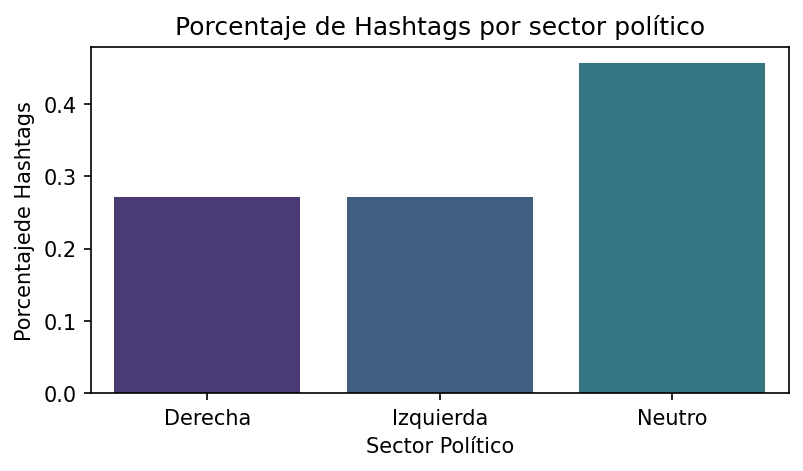
\includegraphics{Images & Logos/EDA/Cantidad de Hashtags por sector politico.png}
	\caption{Porcentaje de Hashtags según la orientación política asignada}
	\label{figure:tweets_cantidad_hashtags}
\end{figure}

De manera similar, la Figura \ref{figure:tweets_porcentaje} muestra la distribución de los tweets según la orientación política asignada a los hashtags asociados. En esta Figura se aprecia que el sector neutro concentra la mayoría de los tweets, con más del 46\%, seguido por la izquierda con un 33\% y finalmente la derecha con cerca de un 29%.

\begin{figure}[!htbp]
	\centering
	\includegraphics{Images & Logos/EDA/Porcentaje de tweets por sector político.png}
	\caption{Porcentaje de Tweets según la orientación política asignada}
	\label{figure:tweets_porcentaje}
\end{figure}

Al analizar la cantidad de tweets por orientación política asignada a lo largo del tiempo, se obtienen los resultados observados en la Figura \ref{figure:tweets_porcentaje_tiempo}, que muestra el porcentaje de tweets de cada día para cada sector, en relación con el total de tweets dicho sector. Se puede notar que algunas fechas resultaron particularmente importantes: el 24 de mayo fue un día de debate y destaca el sector neutro, el 29 de mayo fue el día de la primera vuelta electoral, destacando los tres sectores, el 9 de junio fue cuando se divulgaron los llamados "Petro videos", unos videos filtrados que mostraban discusiones políticas del equipo de campaña de Petro, sobresaliendo la derecha. Además, las fechas cercanas al 19 de junio, día de la segunda vuelta, también presentan un aumento en la actividad y destacan los tres sectores.




\begin{figure}[!htbp]
	\centering
	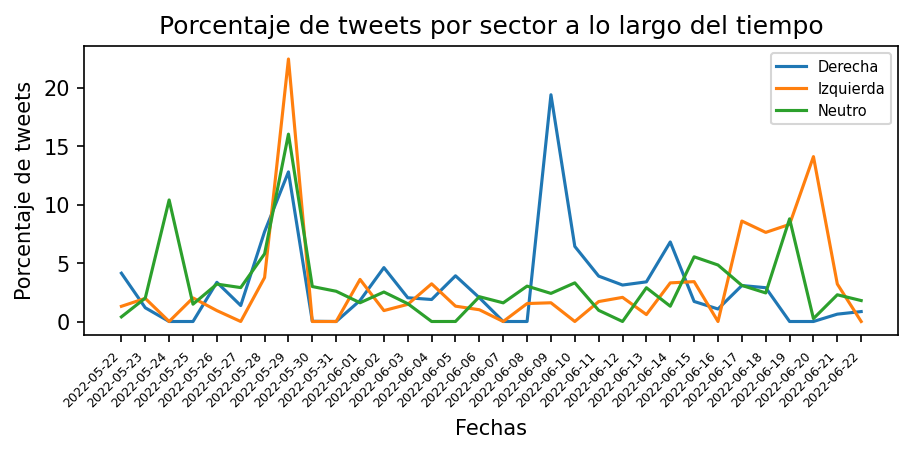
\includegraphics{Images & Logos/EDA/Porcentaje de tweets por sector a lo largo del tiempo.png} 
	\caption{Porcentaje de tweets según orientación política a lo largo del tiempo}
	\label{figure:tweets_porcentaje_tiempo}
\end{figure}



\subsection{Etiquetado}


Se procedió a etiquetar manualmente un conjunto de 1200 tweets seleccionados mediante una muestra aleatoria estratificada proporcional a la cantidad de tweets presentes en los hashtags. Las etiquetas asignadas a cada tweet correspondieron a las emociones identificadas en los mismos.

Una emoción, según la definición de la APA en su Diccionario de Psicología  \citep{vandenbos2007apa}, es un patrón complejo de reacción que involucra elementos experienciales, conductuales y fisiológicos. A través de estos elementos, un individuo intenta abordar un asunto o evento que tiene significado personal. La cualidad específica de la emoción, como el miedo o la ira, está determinada por el significado particular que el individuo atribuye al evento. Por ejemplo, si el evento implica una amenaza, es probable que se genere miedo. Las emociones consisten en tres componentes distintos: una experiencia subjetiva, una respuesta fisiológica y una respuesta conductual o expresiva.

Dentro del contexto de este trabajo, los componentes de experiencia subjetiva y respuesta fisiológica no son accesibles. Por lo tanto, el enfoque principal durante el proceso de etiquetado se centró en la respuesta expresiva, específicamente en cómo el autor del tweet comunica a través del texto la respuesta emocional generada hacia la entidad a la cual va dirigido el tweet.

El proceso de etiquetado consistió en asignar emociones a un tweet a la vez, utilizando una plataforma de etiquetado con un esquema de selección múltiple. Se permitía asignar una o varias emociones al tweet, siguiendo las directrices establecidas en el manual de etiquetado \footnote{\url{https://docs.google.com/document/d/1hoUYKMaYHSeGeOQ2FqRVyahTin6T09Mu8wtl_HY62O0/edit?usp=sharing}}. Esta tarea fue llevada a cabo por el autor y los directores, generando así tres etiquetas independientes para cada tweet.

Para el esquema de etiquetado, se tomó como referencia el enfoque de \cite{mohammad2015sentiment}, en el cual el etiquetador responde varias preguntas y, al ser preguntado sobre la emoción presente en el tweet, puede seleccionar entre 19 emociones distintas. En este trabajo, después de una prueba iterativa para elegir las etiquetas más adecuadas, se llegó a la elección de 14 emociones posibles, además de la categoría "Otra". Estas emociones incluyen alegría, agrado, confianza, admiración, miedo, incertidumbre, sorpresa, asombro, tristeza, decepción, asco, desagrado, ira, odio y otra. En el Cuadro \ref{table:emotions_description} se presenta una descripción detallada de las emociones seleccionadas, basada en definiciones encontradas en el Diccionario de Psicología de la APA, el Diccionario de Oxford \footnote{\url{https://www.oed.com}}, el de la RAE \footnote{\url{https://www.rae.es/}} y Wikipedia \footnote{\url{https://www.wikipedia.org/}}.

\tiny
\begin{longtable}{{ | l | p{13cm} |}}
\caption{Descripción de las emociones usadas} \label{table:emotions_description} \\
\toprule
Emoción & Descripción \\
\midrule
\endfirsthead
\caption[]{Descripción de las emociones usadas} \\
\toprule
Emoción & Descripción \\
\midrule
\endhead
\midrule
\multicolumn{2}{r}{Continued on next page} \\
\midrule
\endfoot
\bottomrule
\endlastfoot
Admiración & La admiración es una emoción social que se siente al observar a personas de competencia, talento o habilidad que superan los estándares. La admiración facilita el aprendizaje social en grupos. La admiración motiva la superación personal a través del aprendizaje de los modelos a seguir. \\
Agrado & Sensación moderada de felicidad o placer que siente una persona por algo que le gusta. \\
Confianza & La confianza implica que una parte se vuelve vulnerable ante otra, asumiendo que esta actuará en su beneficio.En una relación de confianza, el que confía no controla las acciones del otro. \\
Alegría & Es una emoción positiva que suele ir acompañada de bienestar. Se genera como resultado de un evento positivo. \\
Incertidumbre & La incertidumbre es la falta de seguridad, de confianza o de certeza sobre algo. Aparece en situaciones en las que no tenemos control total, en las que nos faltan respuestas e información, y nos puede generar inquietud, inseguridad, estrés, ansiedad e incluso miedo \\
Miedo & El miedo surge ante amenazas reales o imaginarias de daño físico, emocional o psicológico. En textos, se muestra como amenazas hacia el autor del mensaje o lo que se menciona, cuando está vulnerable o en desventaja.  \\
Asombro & La condición de estar asombrado; un estado de asombro abrumador, como por sorpresa o miedo repentino, horror o admiración.  \\
Sorpresa & Se define como una reacción provocada por algo inesperado, extraño o novedoso para la persona. En el texto está principalmente asociada a resultados inesperados o descubrimientos singulares respecto al enunciado del tweet. \\
Decepción & La decepción es la insatisfacción que sigue al fracaso de expectativas o esperanzas. A diferencia del arrepentimiento que se centra en elecciones personales, la decepción se enfoca en el resultado en sí. Puede generar estrés psicológico. \\
Tristeza & La tristeza es un dolor emocional causado por decadencia espiritual, manifestándose en llanto, abatimiento, falta de apetito, cansancio, etc. Ocurre cuando las expectativas no se cumplen o las circunstancias son dolorosas.  \\
Desagrado & Una actitud o un sentimiento de disgusto o aversión. \\
Asco & Contiene una serie de estados con intensidades variables que van desde una leve aprensión hasta una intensa repulsión. Todos los estados de asco se desencadenan por la sensación de que algo es aversivo, repulsivo y/o tóxico.  \\
Odio & El odio es una intensa respuesta emocional negativa hacia ciertas personas, cosas o ideas, generalmente relacionadas con la oposición o repulsión hacia algo. El odio a menudo se asocia con intensos sentimientos de ira, desprecio y disgusto. \\
Ira & La ira surge por objetivos no alcanzados o trato injusto, pudiendo ser peligrosa y relacionada con la violencia. En el texto, el autor reta o reclama por un derecho vulnerado, buscando justicia. \\
\end{longtable}

\normalsize



Este etiquetado se llevo a cabo usando la plataforma web Label Studio \footnote{\url{https://labelstud.io/}} que fue suministrada para cada uno de los etiquetadores, es decir el autor y los directores, a donde se cargaron los tweets a etiquetar. La plataforma permite definir una interfaz de etiquetado personalizada que es presentada en cada uno de los datos a etiquetar, en este caso, cada tweet. Para definir esta interfaz, se plantearon las preguntas necesarias para poder etiquetar adecuadamente los tweets, basándose en el cuestionario planteado por \cite{mohammad2015sentiment}. Esto se llevo a cabo mediante un proceso iterativo, como se describe en la figura \ref{figure:diagrama}, en donde se plantearon algunas preguntas, se etiquetaron algunos tweets a partir de ellas y basándose en la experiencia de etiquetado y el acuerdo obtenido, se replantaron las preguntas. El resultado final de este proceso fue la interfaz de etiquetado que se puede observar en la Figura \ref{figure:interfaz}. Cabe resaltar que para el caso de las emociones, se permitió al etiquetador asignar múltiples etiquetas a cada tweet. Por otro lado, aun cuando la categoría "Neutro" no se encuentra disponible para ser seleccionada, aquellos tweets para los cuales la pregunta "¿Existe contenido emocional en este tweet?" fue respondida con un "No", fueron catalogados con dicha etiqueta. 

\begin{figure}[!htbp]
	\centering
	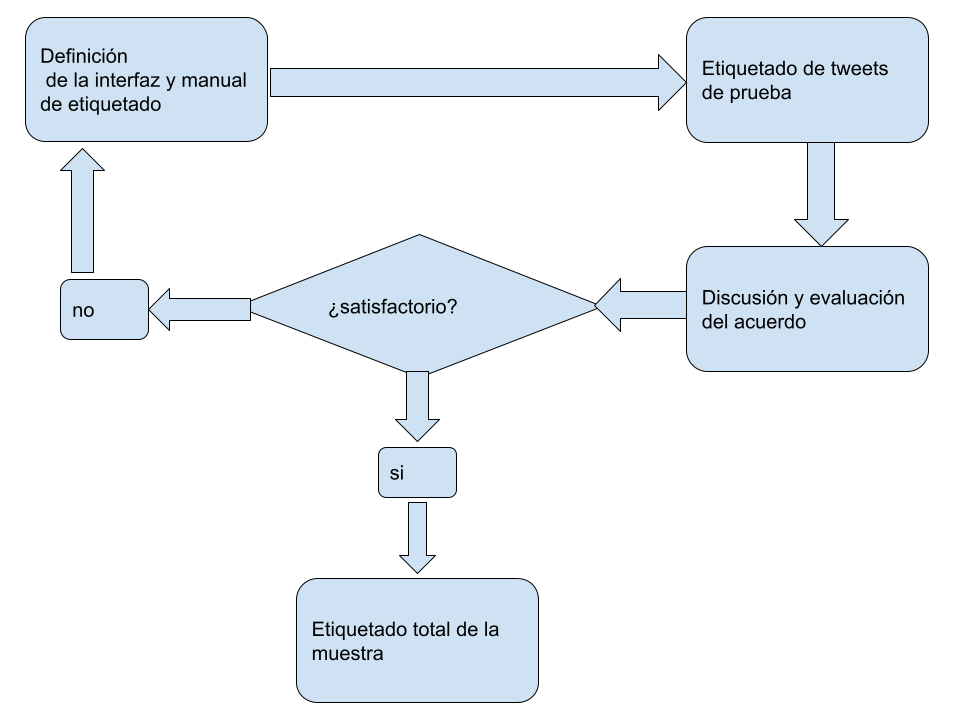
\includegraphics[scale=0.35]{Images & Logos/Diagrama.png}
	\caption{Proceso de etiquetado} 
	\label{figure:diagrama}
\end{figure}

\begin{figure}[!htbp]
	\centering
	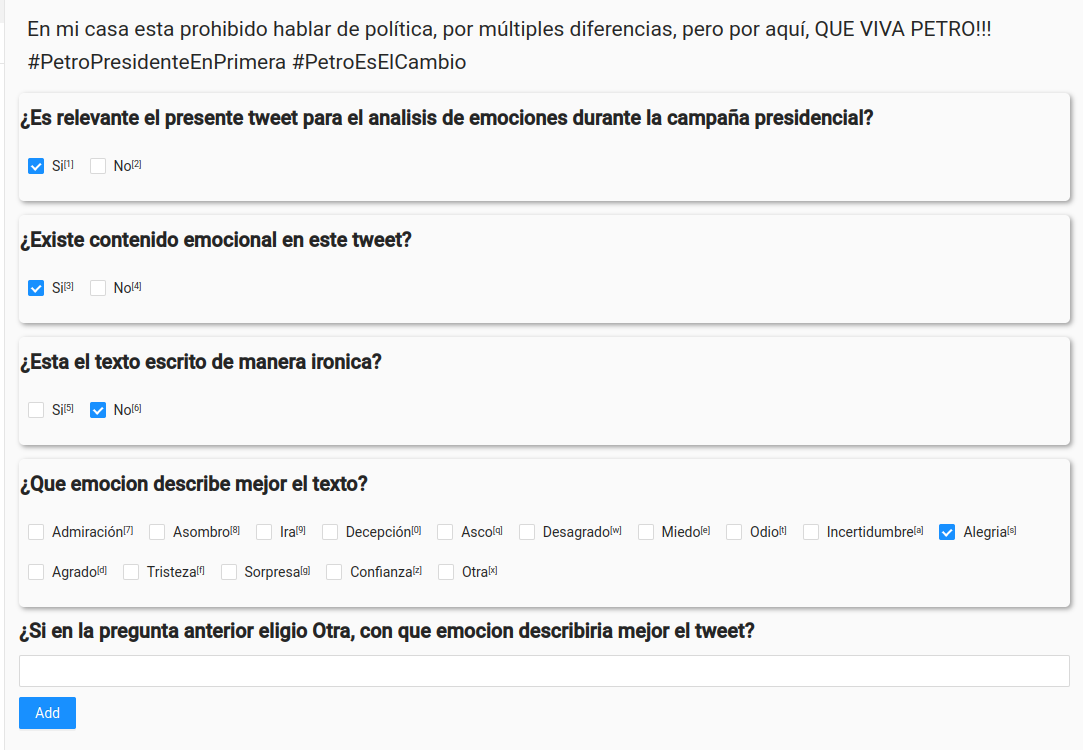
\includegraphics[scale=0.45]{Images & Logos/interfaz.png}
	\caption{Interfaz de etiquetado} 
	\label{figure:interfaz}
\end{figure}


A través del uso de esta interfaz, cada uno de los etiquetadores logro proporcionar sus respuestas las preguntas planteadas para cada uno de los 1200 tweets tomados como muestra. Este proceso produjo una base de datos por etiquetador que al ser consolidadas, permitió calcular la cantidad de tweets etiquetados según la emoción asignada que se observan en el Cuadro \ref{table:tweets_etiquetador}.



\scriptsize
\begin{table}
\centering
\scriptsize
\begin{tabular}{lrrr}
\toprule
Emocion & Cantidad etiquetador 1 & Cantidad etiquetador 2 & Cantidad etiquetador 3 \\
\midrule
Alegria & 61 & 107 & 125 \\
Agrado & 2 & 36 & 59 \\
Confianza & 417 & 242 & 395 \\
Admiración & 79 & 25 & 292 \\
Miedo & 84 & 98 & 76 \\
Incertidumbre & 37 & 28 & 74 \\
Sorpresa & 6 & 3 & 4 \\
Asombro & 1 & 15 & 5 \\
Tristeza & 18 & 10 & 57 \\
Decepción & 137 & 119 & 74 \\
Asco & 82 & 119 & 374 \\
Desagrado & 494 & 357 & 463 \\
Ira & 26 & 111 & 161 \\
Odio & 23 & 0 & 115 \\
Otra & 4 & 11 & 21 \\
Neutro & 107 & 111 & 115 \\
\bottomrule
\end{tabular}
\caption{Cantidad de tweets asignados a cada emocion por etiquetador}
\label{table:tweets_etiquetador}
\end{table}

\normalsize


Al analizar las etiquetas asignadas por los etiquetadores, se encontró que estos asignaban etiquetas diferentes pero que estaban cercanas en un sentido semántico a algunos tweets. Para poder cuantificar esta situación, se procedió a calcular la correlación que tuvieron las etiquetas asignadas por los etiquetadores, obteniendo así los resultados observados en la Figura \ref{figure:correlacion_emociones}  

\begin{figure}[!htbp]
	\centering
	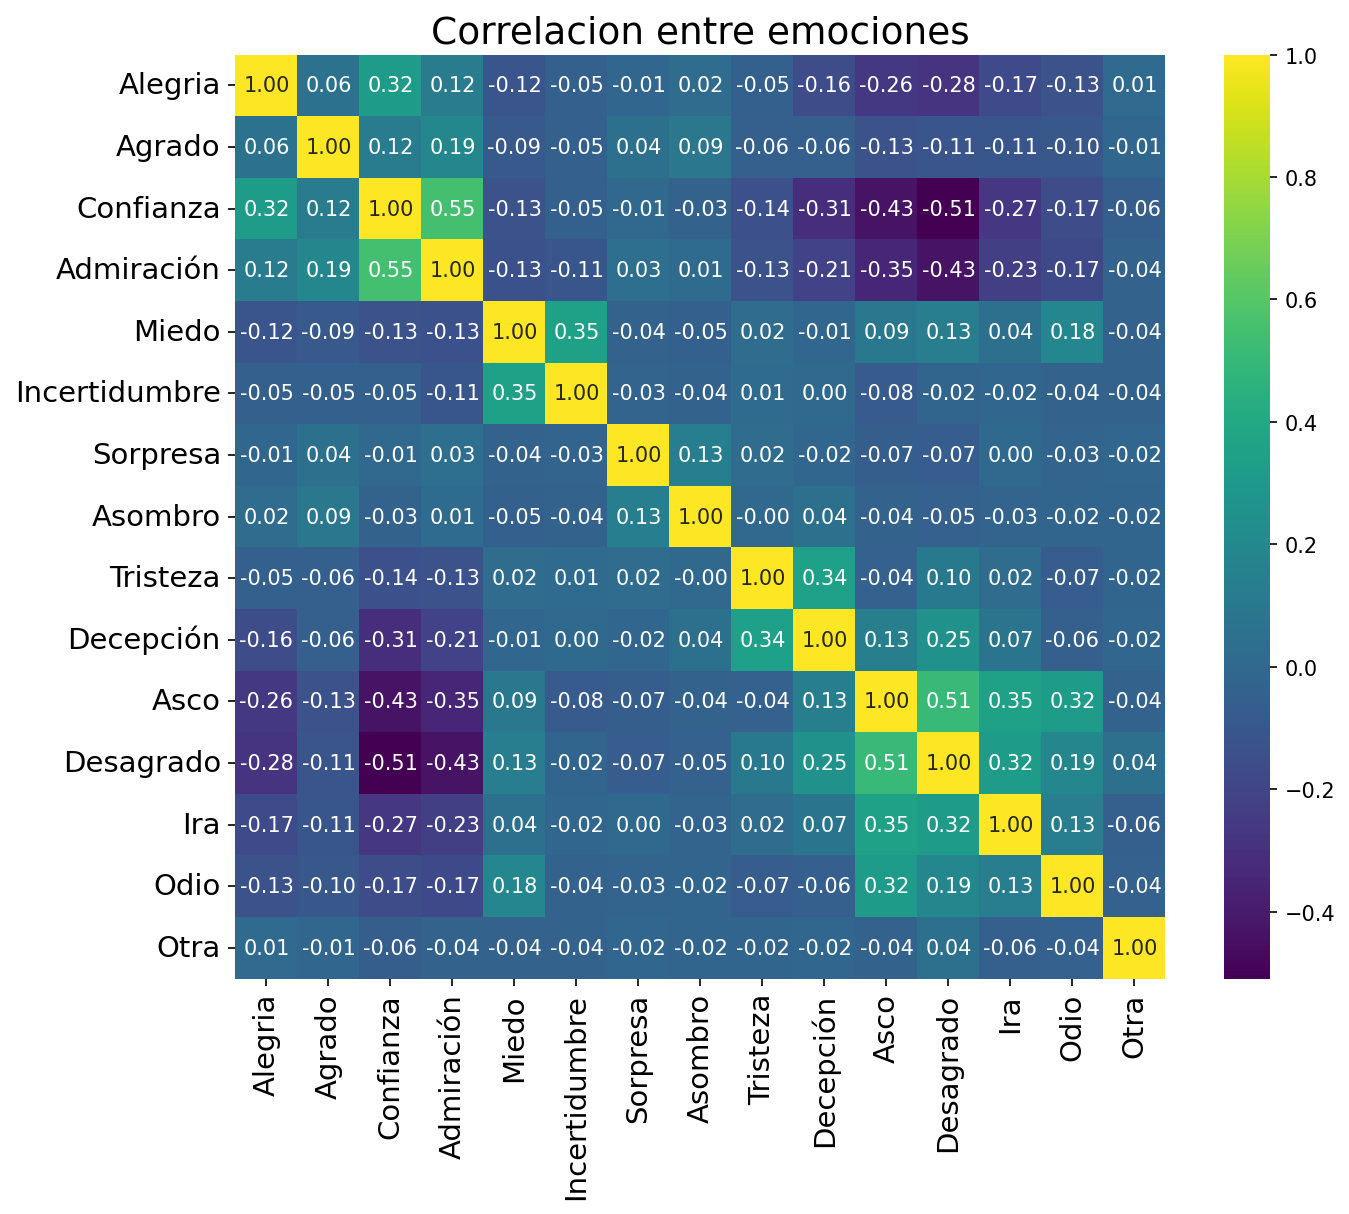
\includegraphics[scale=0.65]{Images & Logos/EDA/emotions_correlations.png} 
	\caption{Indice de correlación entre etiquetadores de las emociones asignadas a los tweets}
	\label{figure:correlacion_emociones}
\end{figure}


Estos resultados llevaron a una conclusión similar a la planteada por \cite{mohammad2015sentiment}, donde resulta útil agrupar las etiquetas iniciales de manera que aquellas con cercanía semántica y, por ende, una correlación considerable en los resultados obtenidos, sean asignadas a un mismo grupo. En este sentido, se construyeron las siguientes 4 etiquetas agrupadoras: Alegría, que incluye las etiquetas Alegría, Agrado, Confianza y Admiración; Miedo, que incluye las etiquetas Miedo e Incertidumbre; Tristeza, que incluye las etiquetas Tristeza y Decepción; y Asco, que incluye las etiquetas Asco, Desagrado, Ira y Odio. Por otro lado, si bien las etiquetas sorpresa y asombro presentan una leve correlación, estas fueron descartadas a que fueron muy pocos tweets a los que les fue asignadas alguna de estas etiquetas.

Para asignar las etiquetas finales a los tweets, se empleó el mismo sistema utilizado por \cite{mohammad2015sentiment}, donde más de la mitad de los etiquetadores debían estar de acuerdo en una etiqueta específica para que esta pudiera ser asignada. De esta manera, cada etiqueta agrupadora se asignó a un tweet si al menos dos de los etiquetadores le habían asignado alguna de las etiquetas que la componen. Además, debido a que se permitió a los etiquetadores asignar múltiples etiquetas a cada tweet, esto permitió la asignación de más de una etiqueta agrupadora.

El acuerdo observado entre los etiquetadores para cada una de estas 4 etiquetas agrupadoras se midió utilizando el índice de Fleiss Kappa \citep{fleiss1971measuring}. Los resultados se presentan en el Cuadro \ref{table:agreements}. Se puede observar que a la gran mayoría de los tweets se les asignó las etiquetas de Asco y Alegría con 464 y 580 tweets respectivamente.

\begin{table}
\caption{Indice de Fleiss Kappa en cada emocion}
\label{table:agreements}
\centering
\begin{tabular}{lllll}
\toprule
 & alegria & miedo & tristeza & asco \\
\midrule
Cantidad de Tweets & 464 & 98 & 103 & 580 \\
Indice de Fleiss Kapp & 0.69 & 0.47 & 0.4 & 0.62 \\
\bottomrule
\end{tabular}
\end{table}


Se aprecia así mismo cómo Alegría y Asco tuvieron puntajes relativamente altos en comparación con Tristeza y Miedo. Esto se explica en parte por la cercanía que estas dos últimas tienen con Asco, como se puede ver en el tweet número 1 del Cuadro \ref{table:ejemplos_etiquetador}. En él, dos de los etiquetadores coincidieron en asignar emociones relacionadas con Tristeza, mientras que el tercero asignó emociones relacionadas con Asco. Este mismo fenómeno ocurre con Miedo, como se aprecia en el tweet número 2 del Cuadro. Allí también fue el caso en que uno de los etiquetadores asignó emociones relacionadas con Asco, mientras que los otros dos asignaron emociones relacionadas con Miedo.

\scriptsize
\begin{table}[t]
\scriptsize
\begin{tabular}{{ | p{1.5cm}| p{7cm} | p{1.5cm} | p{1.5cm} | p{1.5cm} |}}
\hline
Numero de Ejemplo & Tweet & Etiquetador 1 & Etiquetador 2 & Etiquetador 3 \\
\hline
1 & \#LoPeorDeEstasElecciones es la división de la gente  de este país esta gente y cosas ya que pasan & Decepción & Decepción & Desagrado \\
2 & @Zuletalleras Son 4 años O es la. Derecha va realizar un golpe de estado? No cree a sus comentarios son ofensivos e incendiarios.... \#PetroEsPresidente & Miedo, Incertidumbre & Miedo & Asco, Desagrado \\
\hline
\end{tabular}
\caption{Ejemplos de tweets clasificados por etiquetador}
\label{table:ejemplos_etiquetador}
\end{table}

\normalsize

La coincidencia en las etiquetas finales asignadas a los tweets , se puede observar en la Figura \ref{figure:Matriz_etiquetas}, donde se representa la co-ocurrencia de estas. En esta Figura, se destaca que la etiqueta de asco fue la que se asignó conjuntamente con mayor frecuencia a todas las demás etiquetas.

\begin{figure}[!htbp]
	\centering
	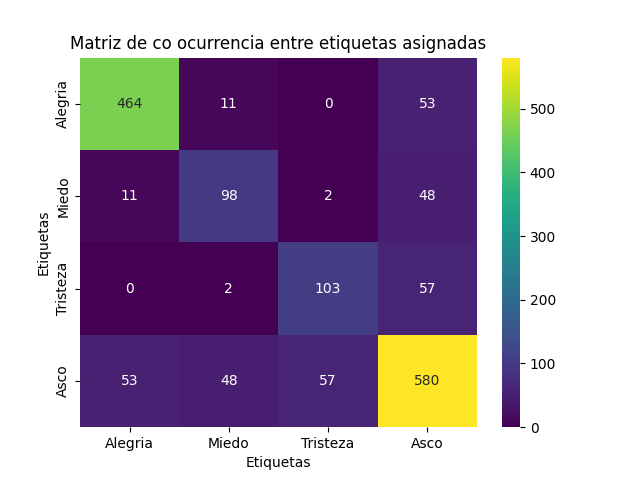
\includegraphics[scale=0.75]{Images & Logos/Results/Matriz_confusion_labels.png}
	\caption{Matriz de co ocurrencia entre etiquetas asignadas}
	\label{figure:Matriz_etiquetas}
\end{figure}

En este contexto, el Cuadro \ref{table:labels_counts} presenta la cantidad de tweets etiquetados con diferentes números de etiquetas. Los tweets con cero etiquetas corresponden a casos en los que los etiquetadores coincidieron en la ausencia de contenido emocional o hubo falta de acuerdo en la asignación de etiquetas. Es notable que la mayoría de los tweets se etiquetaron con una sola etiqueta, aunque también hay una cantidad significativa con múltiples etiquetas.

\begin{table}[!htbp]
\centering
\begin{tabular}{rr}
\toprule
Cantidad de etiquetas & Cantidad de Tweets \\
\midrule
0 & 123 \\
1 & 909 \\
2 & 165 \\
3 & 2 \\
\bottomrule
\end{tabular}
\caption{Cantidad de tweets por cantidad de etiquetas finales asignadas}
\label{table:labels_counts}
\end{table}


En el Cuadro \ref{table:ejemplos_multples} se presentan algunos ejemplos de tweets con múltiples etiquetas en la asignación final. Por ejemplo, el primer tweet comparte las etiquetas de alegría y asco debido a que el autor refleja diferentes emociones en frases distintas del tweet. Además, hay casos en los que una misma frase o todo el contenido del tweet refleja múltiples emociones para los etiquetadores. Tal es el caso de los ejemplos 2 y 3, que comparten las etiquetas de tristeza y asco, así como el ejemplo 4, que comparte las etiquetas de miedo y asco.

\scriptsize
\begin{table}[!htbp]
\scriptsize
\begin{tabular}{{| p{1.5cm} | p{11.5cm} | p{1cm} |}}
\hline
Numero de Ejemplo & Tweet & Etiquetas \\
\hline
1 & En \#ElDebateDefinitivo Fajardo con sus preguntas hizo subir de votos a @petrogustavo en los votos de los indecisos. La ausencia del ingeniero ayudó a Petro, Fico pierde sólo. \#PetroGanaDebate, es el único candidato que gana con argumentos. & alegria, asco \\
2 & Comenzo el entrampamiento público en el debate presidencial. Ya ni disimulan. \#ElDebateDefinitivo & tristeza, asco \\
3 & Fajardo quedo tan peinado que ya se quiere ir \#ElDebateDefinitivo & tristeza, asco \\
4 & En conclusión \#ElDebateDefinitivo deja claro que Petro es un peligro. Mentiroso, arrogante, tramposo, encubridor, manipulador, violento, pasivo agresivo, resentido. En resumen, una porquería de ser humano, qué digo humano... un demonio.  Petro es el Pol Pot de Ciénaga de Oro & miedo, asco \\
\hline
\end{tabular}
\caption{Ejemplos de tweets con etiquetas múltiples}
\label{table:ejemplos_multples}
\end{table}

\normalsize


\section{Experimentos de clasificación}



En esta sección, se aborda la descripción, entrenamiento y evaluación de modelos de lenguaje preentrenados. Dado que la tarea principal de este trabajo es analizar las emociones presentes en tweets escritos en español, se han seleccionado seis modelos diferentes debido a su relevancia para dicha tarea. Cada modelo se describe de manera concisa, y se explican las herramientas utilizadas tanto para el entrenamiento como para el almacenamiento de los resultados. Además, se detalla la división de los datos realizada y se mencionan las métricas elegidas para evaluar el entrenamiento y el rendimiento de los modelos en el conjunto de test.

\subsection{Modelos preentrenados}

Los modelos de lenguaje preentrenados se encuentran disponibles para su uso en la plataforma Hugging Face \footnote{\url{https://huggingface.co/}}, utilizando la librería Transformers \footnote{\url{https://huggingface.co/docs/transformers/index}}. A partir de esta plataforma, y considerando la pertinencia de los modelos para la tarea en cuestión, se han seleccionado seis modelos distintos para ser evaluados y escoger aquel que muestre el mejor desempeño. Los modelos elegidos son RoBERTuito \citep{perez-etal-2022-robertuito}, BERTIN \citep{BERTIN}, BETO \cite{CaneteCFP2020}, ELECTRICIDAD \cite{mromero2020electricidad-base-discriminator}, RoBERTa \cite{ROBERTA} y twitter-XLM \cite{barbieri2022xlm}. En el Cuadro \ref{table:model_description}, se proporciona una breve descripción de cada uno de estos modelos.


\scriptsize
\begin{table}
\caption{Descripción de los modelos usados}
\label{table:model_description}
\begin{tabular}{{ | l | l | p{7cm} |}}
\toprule
Modelo & Localizacion & Descripcion  \\
\midrule
robertuito  & pysentimiento/robertuito-base-uncased & Modelo de lenguaje preentrenado para contenido generado por usuarios en español, entrenado siguiendo las pautas de RoBERTa en 500 millones de tweets. \\
bertin & bertin-project/bertin-roberta-base-spanish & Modelo basados en RoBERTa entrenados desde cero en la parte española de mC4 usando Flax \\
electricidad & mrm8488/electricidad-base-discriminator & Electricidad-base-discriminator es un modelo base tipo Electra entrenado en un gran corpus español (también conocido como corpus de BETO) \\
beto & dccuchile/bert-base-spanish-wwm-cased & BETO es un modelo BERT formado en un gran corpus español. BETO tiene un tamaño similar a un BERT-Base y fue entrenado con la técnica de enmascaramiento de palabras completas. \\
roberta & PlanTL-GOB-ES/roberta-base-bne & El roberta-base-bne se basa en el modelo base de RoBERTa y ha sido preentrenado utilizando un corpus en español de 570 GB de texto limpio  \\
twitter-xlm & cardiffnlp/twitter-xlm-roberta-base & Este es un modelo basado en XLM-roBERTa multilingüe entrenado en ~198 millones de tweets y ajustado para el análisis de sentimientos. \\
\bottomrule
\end{tabular}
\end{table}

\normalsize



\subsection{Entrenamiento de los modelos}


Debido a que el fine-tuning de estos modelos requiere una gran capacidad de cómputo, se decidió utilizar el servicio de Google Colab \footnote{\url{https://colab.research.google.com/}}, donde es posible desarrollar notebooks haciendo uso gratuito de GPUs. Allí, se empleó la librería Transformers de Hugging Face para acceder a los modelos.

Para entrenar los modelos, se realiza una transformación de los datos de entrada en vectores tokenizados que puedan ser interpretados por el modelo. Estos datos transformados se suministran al modelo junto con los hiperparámetros y la métrica de evaluación a utilizar.

Los principales hiperparámetros empleados incluyen la implementación de AdamW, un algoritmo de optimización propuesto por \cite{loshchilov2017decoupled}. Se utilizo asi mismo un learning rate de 5e-05. Además, se realizaron 3 épocas de entrenamiento en el conjunto de entrenamiento y se utilizó un batch size de 8.

\subsection{Evaluación de los modelos}

Los modelos fueron entrenados y evaluados utilizando  el promedio Micro de la metrica F1 score. F1 score esta definida de la siguiente manera:


\[
{\text{F1}}=\frac{\text{TP} }{\text{TP} + \frac{1}{2}\text{(FP +FN)}}
\]

Donde TP es el número de verdaderos positivos, FP es el número de falsos positivos y FN es el número de falsos negativos en todas las clases. El Micro F1 score se calcula de la misma, pero teniendo en cuenta todas las clases presentes. Esta métrica fue elegida debido a que el modelo permite la clasificación múltiple, y con ella se puede evaluar el desempeño de las distintas clases simultáneamente.

Para entrenar y evaluar los modelos, se empleo el método Monte Carlo Cross Validation, en donde cada modelo es entrenado múltiples veces con ligeras variaciones en el tamaño de los conjuntos de train y test, entrenando así diez veces cada modelo, registrando cada vez los resultados de su desempeño. Esto se hizo para obtener una medición más robusta, dada la naturaleza aleatoria de las redes neuronales.Se optó por no realizar una tercera partición debido a que no se llevó a cabo una optimización de los hiperparámetros, además del tamaño del conjunto de datos etiquetados. Los resultados de entrenamiento de cada modelo se registraron en la plataforma Wandb \footnote{\url{https://wandb.ai/}}, una herramienta de seguimiento de modelos. Los detalles pueden observarse en el informe del proyecto creado en dicho sitio \footnote{\url{https://api.wandb.ai/links/juanjose_if3/mtzaowe2}}.






